\section{Theory}

\subsection{The Transmission electron microscope}
The Transmission electron microscope (TEM) is a microscope that far exceeds the capabilities of a normal light microscope. Both types of microscope use a series of lenses to magnify the image of a specimen.
A normal light microscope can amplify an image up to about 1500$\times$ and is limited by the diffraction limit of light. Assuming an average wavelength of \SI{550}{\nm} for green light, a high-end microscope is limited to resolving features \SI{100}{\nm} apart.
This limit is insufficient for looking at atomic structures \cite{PhysRevLett.106.193905}.\\
An electron microscope circumvents this limit by using electrons, not light, to probe the specimen. Electrons when accelerated have a smaller wavelength than light thus allowing for images with resolved features as small as \SI{0.05}{\nm}. \cite{kisielowski_freitag_bischoff_van}
The TEM works by releasing electrons from an electron source and accelerating them to an energy typically expressed in kilo-electronvolt; as shown in equation \ref{eq:acc_volts}, the higher the accelerating voltage of the microscope the smaller the de Broglie wavelength of an electron, which results in a higher resolving power. Modern electron microscopes accelerate electrons up to \SI{300}{\kilo \electronvolt}

\begin{equation}
    \lambda_e = h\cdot \left[ 2 \cdot e \cdot m_e \cdot V_a \right]^{-1/2}
    \label{eq:acc_volts}
\end{equation}

\begin{figure}[h]
    \centering
    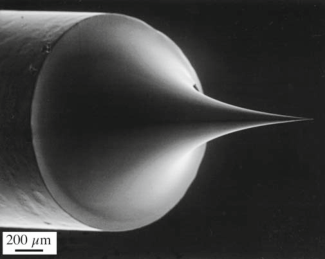
\includegraphics[keepaspectratio, width=0.5\linewidth]{resources/Figures/feg.png} 
    \caption{Pictured is the tip of a field emission gun \cite{Williams2009-ww}. The tapered tip facilitates the creation of a strongly varying potential that eases the expulsion of electrons from the material. These electrons are then accelerated along the optical axis.}
    \label{fig:feg}
\end{figure}

In a TEM the electrons are released from a field emission gun (FEG, pictured in Figure \ref{fig:feg}). 
The FEG is placed in proximity to two anodes, the first anode is positively charged to several kilovolts such that it extracts electrons from the tip of the FEG, the second anode is charged to the wanted acceleration voltage \cite{Williams2009-ww}.
FEGs are about three orders of magnitude brighter than thermionic emission electron sources \cite{field-emission}.
After being emitted the electrons pass through a monochromator that reduces the energy spread of the emitted electrons. An electron then continues along the optical axis into an illuminating system consisting of multiple electromagnetic lenses, which lenses are activated and to what extent depends on the operating mode of the electron microscope.

% \subsubsection{Bright Field}
% A bright field (BF) image of the sample is acquired by using a parallel electron beam. This beam is formed using the lens configuration shown in figure \ref{fig:tem_operating}. This parallel beam is typically several micrometers in size at magnifications up to 20k-100k$\times$.
% In normal operating mode a BF image is captured by a camera looking at a phosphorous screen or by a camera directly, this method of imaging is most analogues to a normal light microscope.
% The electron beam is focused in such a way that it illuminates the sample with a parallel beam, such a beam is also used for creating the clearest diffraction patterns.
% %A bright field image can also be formed in STEM operating mode.
% \begin{figure}[h]
%     \centering
%     \def\svgwidth{.66\linewidth}
%     \import{resources/Figures}{parallel_op_mode.pdf_tex}
%     \caption{Illumination system for parallel beam.}
%     \label{fig:tem_operating}
% \end{figure}
\subsubsection{Dark Field, Z-contrast}
For dark field and Z-contrast the electron beam is focused to a small area, this creates a higher intensity electron beam with a probe-like point as can be seen in Figure \ref{fig:stem_operating}. Since all the electrons are focused on a small area there is no contrast information that can be used to form an image. To form an image using such a beam the probe point needs to be scanned over the sample leading to the term Scanning Transmission Electron Microscopy.
Dark field images use electrons scattered away from the optical axis to form an image, to achieve this most STEMs have a series of annular dark field detectors.
These ring shaped detectors encircle the central bright field detector and can collect electrons that have been scattered at various angles. Normal dark field detectors collect electrons scattered up to an angle of \SI{50}{\milli \radian}. The outermost detector is the high-angle annular dark field detector (HAADF) which collects electrons scattered beyond \SI{50}{\milli \radian} and can be used to create Z-contrast (atomic number Z) or mass-thickness images.
The HAADF detector is used since the electrons it collects are almost exclusively incoherently elastically scattered which is proportional to the atomic number Z.
The scanning beam then gathers this atomic number information as intensity information for every probe position in the sample.
Layering two monolayers such that the atoms are aligned, and the probe is perpendicularly incident on the sample will sum the intensity of the two atomic weights of the stacked atoms in the image. The stacking pattern can then be determined by looking at a line plot of the atomic mass over atoms.  
\begin{figure}[h]
    \centering
    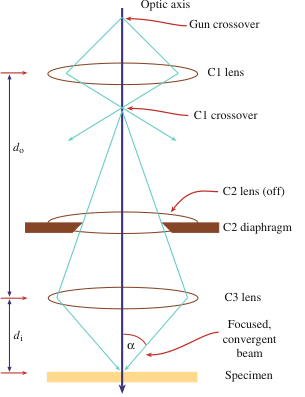
\includegraphics[width=0.5\textwidth, keepaspectratio]{resources/Figures/stem_operating.png}
    \caption{Illumination system for convergent beam.}
    \label{fig:stem_operating}
\end{figure}

% \subsubsection{Energy-dispersive x-ray spectroscopy}
% %Pagina 581 W\&C
% \begin{minipage}[h]{0.6\linewidth}
%         \def\svgwidth{0.66\linewidth}
%         \import{resources/Figures}{Titan_full_column.pdf_tex}
%         \captionof{figure}{Cross-section of an aberration corrected electron microscope}
%         \label{fig:tem_crossection}
% \end{minipage}


\subsection{Transition-metal dichalcogenides and their crystal structure}
\subsubsection{Transition metal dichalcogenides}
Transition metal dichalcogenides or TMDCs are a family of materials consisting of transition metals (group 3 through 12 on the periodic table) and chalcogen atoms (Sulphur, Selenium or Tellurium) in an \ce{MX_2}-configuration, where \ce{M} is the metal atom and \ce{X_2} are the chalcogen atoms \cite{C7TA04268J}.
The properties of TMDCs depend greatly on the amount of stacked layers and with individual layers being as thin as \SI{6.5}{\angstrom} for \ce{MoS_2} these materials are often referred to as layered or two-dimensional materials.
Decreasing the amount of layers from bulk changes electrical properties such as the bandgap which for some TMDCs can go from an indirect to a direct bandgap.
These electrical properties make TMDCs useful in electronics as transistors and in optoelectronics as emitters and detectors \cite{emerg_photolum, LopezSanchez2013, Radisavljevic2011}. 
If present, multiple layers of TMDCs are held together by weak interlayer Van der Waals forces making these materials flexible and transferable using polymer based techniques \cite{reganEmergingExcitonPhysics2022a}.

\subsubsection{Crystal lattice}
An infinitely repeating group of atoms is called an ideal crystal, such a crystal is constructed by attaching the same group of atoms, often called a unit cell, to a lattice.
The lattice can be constructed from $n$ independent lattice vectors. $n=1$ for an atomic chain, $n=2$ for a two-dimensional monolayer, and, $n=3$ for a three-dimensional crystal.
If no smaller repeating group of atoms can be constructed to fill the lattice then this group of atoms is called the primitive unit cell and the $n$-independent lattice vectors are then called the primitive translation vectors $a_{n}$ \cite{Kittel1995-qt}.
Each of the $n$ lattice vectors signifies a direction and length of displacement needed such that the shifted crystal lattice is indistinguishable from the original crystal lattice \ref{eq:lattice_equivalent}.
Lattice vectors are also used to specify the orientation of a crystal plane by denoting where the plane intersects the lattice vectors, this procedure allows for unique indexing of crystallographic planes. The use of these planes will be discussed in \ref{sec:diffraction}.
\begin{equation}
    \vec{r}' = \vec{r} + u_1 \vec{a_1} +u_2 \vec{a_2} + u_3 \vec{a_3}
    \label{eq:lattice_equivalent}
\end{equation}

\subsubsection{Reciprocal lattice and electron diffraction}
\label{sec:diffraction}
In the previous section the crystal lattice was introduced, and it was mentioned that there were unique planes characterized by the points where they intersect the lattice vectors.
In reciprocal space every lattice point is equivalent to one set of these planes.
To best understand a crystal, it is helpful to conceptualize it as having two lattices. The first lattice pertains to the organization of the atoms within the crystal's unit cells. The second lattice is a pattern of points that is specific to each crystal and does not correspond to the atom arrangement. Rather, each point in the lattice is linked to a particular set of planes within the crystal \cite{Williams2009-ww}.
Both lattice constructions are equally valid but are helpful under different circumstances; the reciprocal lattice, for instance, is a useful geometrical construct when talking about diffraction.

The reciprocal lattice, just like the crystal lattice, is constructed by vectors; in the case for the reciprocal lattice these are the reciprocal lattice vectors $\vec{b}_n$.
The reciprocal lattice vectors are constructed from the real-space lattice vectors using equation (\ref{eq:lattice_ortho_norm}) and satisfy relation (\ref{eq:lattice_vec_prop}) with their real-space counterpart.
Using these definitions the reciprocal lattice vectors are unique.
Any reciprocal vector can now be composed uniquely by a linear combination of the reciprocal lattice vectors, such that any vector is scaled and summed. If the scalars are integers they are the miller indices and correspond to a crystallographic plane. \\
Scattering off of these planes shows as a series of high-intensity spots in a diffraction pattern image (Figure \ref{fig:diffraction_pattern}), such an image can be taken in the diffraction mode of a scanning transmission electron microscope (STEM). \\

\begin{minipage}{0.5\textwidth}
    \begin{equation}
        \vec{b}_i = 2 \pi \vec{a}_j \times \vec{a}_k \cdot \left[ \vec{a}_i \cdot ( \vec{a}_j \times \vec{a}_k ) \right]^{-1} 
        \label{eq:lattice_ortho_norm}
    \end{equation}
\end{minipage}%
\begin{minipage}{0.5\textwidth}
    \begin{equation}
        \vec{b}_i \cdot \vec{a}_j = 2\pi \delta_{ij}
        \label{eq:lattice_vec_prop}
    \end{equation}
\end{minipage}\\

In a transmission electron microscope the electrons emanating from the field emission gun are modelled as plane waves. When incident on an atomically thin crystalline sample, the plane waves scatter predictably following the physical criteria that incoming and outgoing electrons beams are plane waves with wave vectors $\vec{k_I}$ and $\vec{k_O}$ for incoming and outgoing waves. The resulting change in wave vector due to the scattering of the sample is then equal to $\vec{K} = \vec{k_I}-\vec{k_O}$. As seen in Figure \ref{fig:scatt_angle}, the outgoing electron beam wavefront is deflected by an angle $\theta$ from the incident electron beam such that both are in phase, this angle is the Bragg angle \cite{Williams2009-ww}; and using that $\vert \vec{k_I} \vert = \vert \vec{k_O} \vert = \vert \vec{K} \vert =\lambda_e^{-1}$, with $\lambda_e$ the electron wavelength, the scattering angle can be expressed as:

\begin{equation}
    \sin{\theta}=\frac{\vert \vec{K}\vert / 2}{\vert \vec{k_I}\vert}
    \label{eq:bragg_angle}
\end{equation}

If both outgoing rays from the same incoming beam wavefront are then in phase, meaning that the extra distance travelled by on of the rays is a multiple of the wavelength, it shows as a bright spot in the image and then the following condition is met for the Bragg angle:

\begin{equation}
    n \lambda_e = 2 d \sin{\theta_B}
    \label{eq:bragg_angle_ser}
\end{equation}

This shows that scattering allows for a finite quantized momentum transfer from the electron to the crystal lattice or vice versa. In a crystalline sample this results in bright spots in the diffraction image, where each bright spot can be indexed and attributed to a family of planes in the crystal that facilitate the momentum transfer for the electrons to reach that spot on the detector or phosphor film.
Just as the real-space lattice has a unit cell so does the reciprocal lattice. In reciprocal space this unit cell is called the Brillouin zone.

\begin{figure}
    \centering
    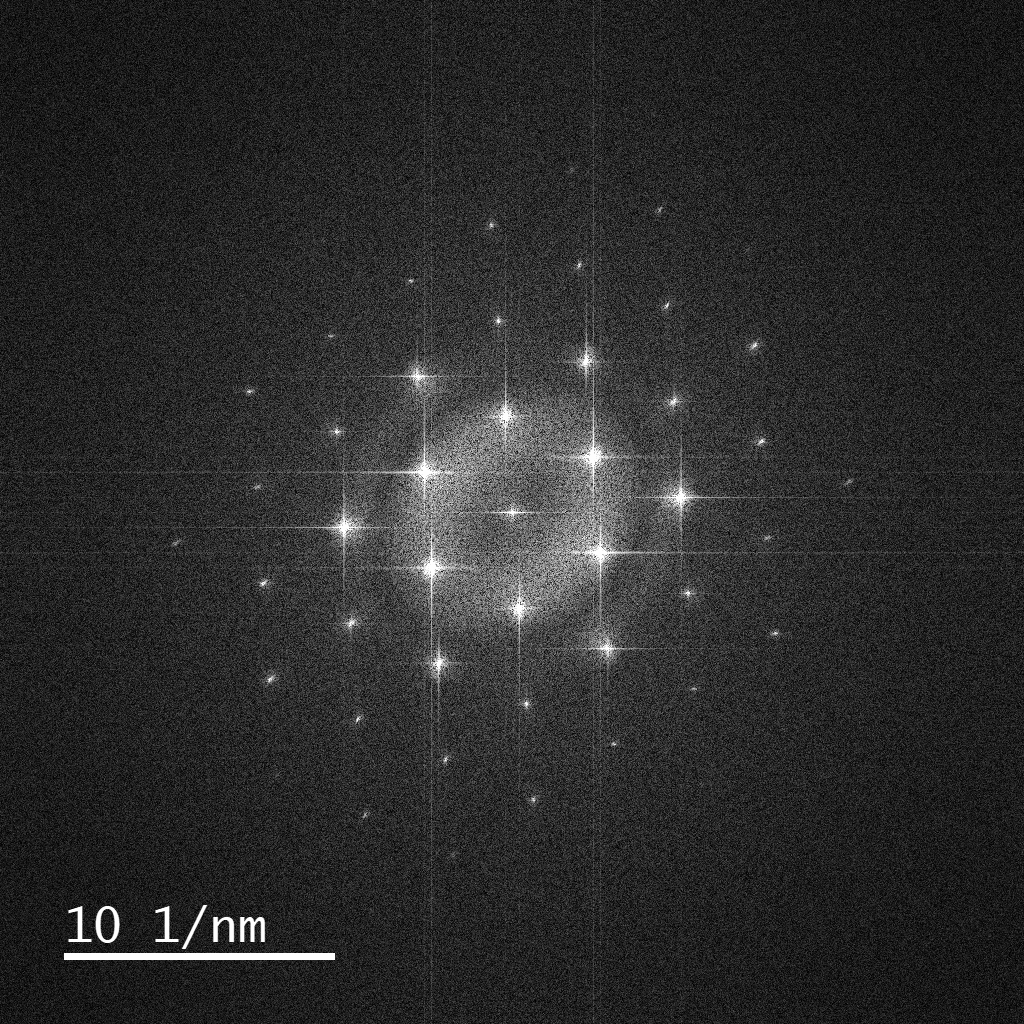
\includegraphics[width=0.3\textwidth, keepaspectratio]{resources/Figures/fft_of_ml.png}
    \caption{Diffraction Pattern}
    \label{fig:diffraction_pattern}
\end{figure}

\begin{figure}
    \centering
    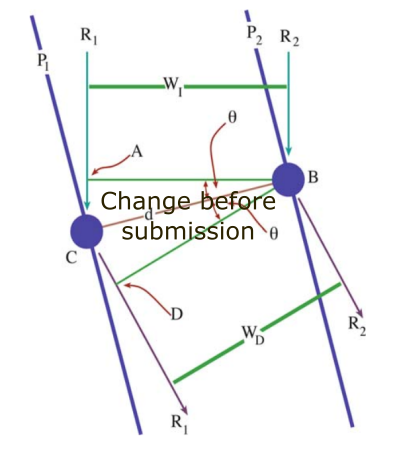
\includegraphics[width=0.3\textwidth, keepaspectratio]{resources/Figures/scattering.png}
    \caption{Scattering diagram}
    \label{fig:scatt_angle}
\end{figure}

\subsubsection{Convergent beam electron diffraction}
In convergent beam electron diffraction the sample is not illuminated by a parallel beam of electrons but instead the electron microscope forms a cone-like shape such that all electrons are focused onto a area only a few atoms wide. The convergence of the electron beam is characterised by the semi-convergence angle $\alpha$ and is usually few to tens of \si{\milli\radian} in size.
Since the local crystal structure is now imaged by a cone-like probe, and not a parallel beam, it is illuminated from multiple different incoming angles; this distribution of incoming angles is then scattered due to the planes in the crystal lattice with the effect of opening the Bragg spots from the previous section to Bragg disks. A typical CBED pattern is displayed in Figure \ref{fig:pacbed}.

\begin{figure}
    \centering
    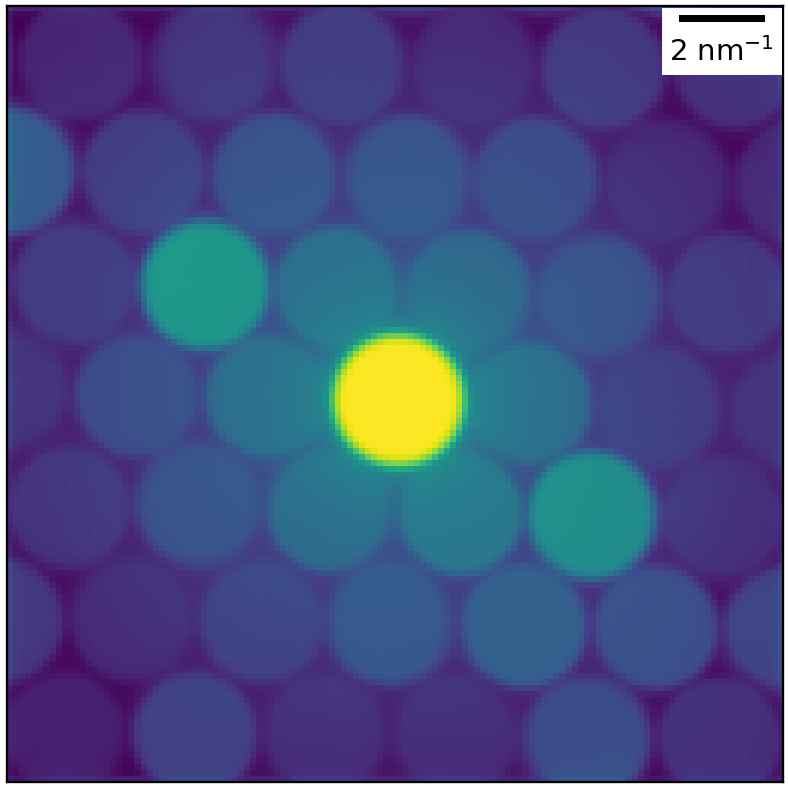
\includegraphics[width=0.5\textwidth, keepaspectratio]{resources/Figures/pacbed_hole.png}
    \caption{A convergent-beam electron diffraction pattern imaged using the EMPAD sensor. Image was calibrated by determining the distance in pixels between Bragg disks and comparing to the FFT of the same crystal imaged using the calibrated CETA camera.}
    \label{fig:pacbed}
\end{figure}

\subsection{Moiré Physics in two-dimensional heterostructures}

\begin{figure}[h]
    \centering
    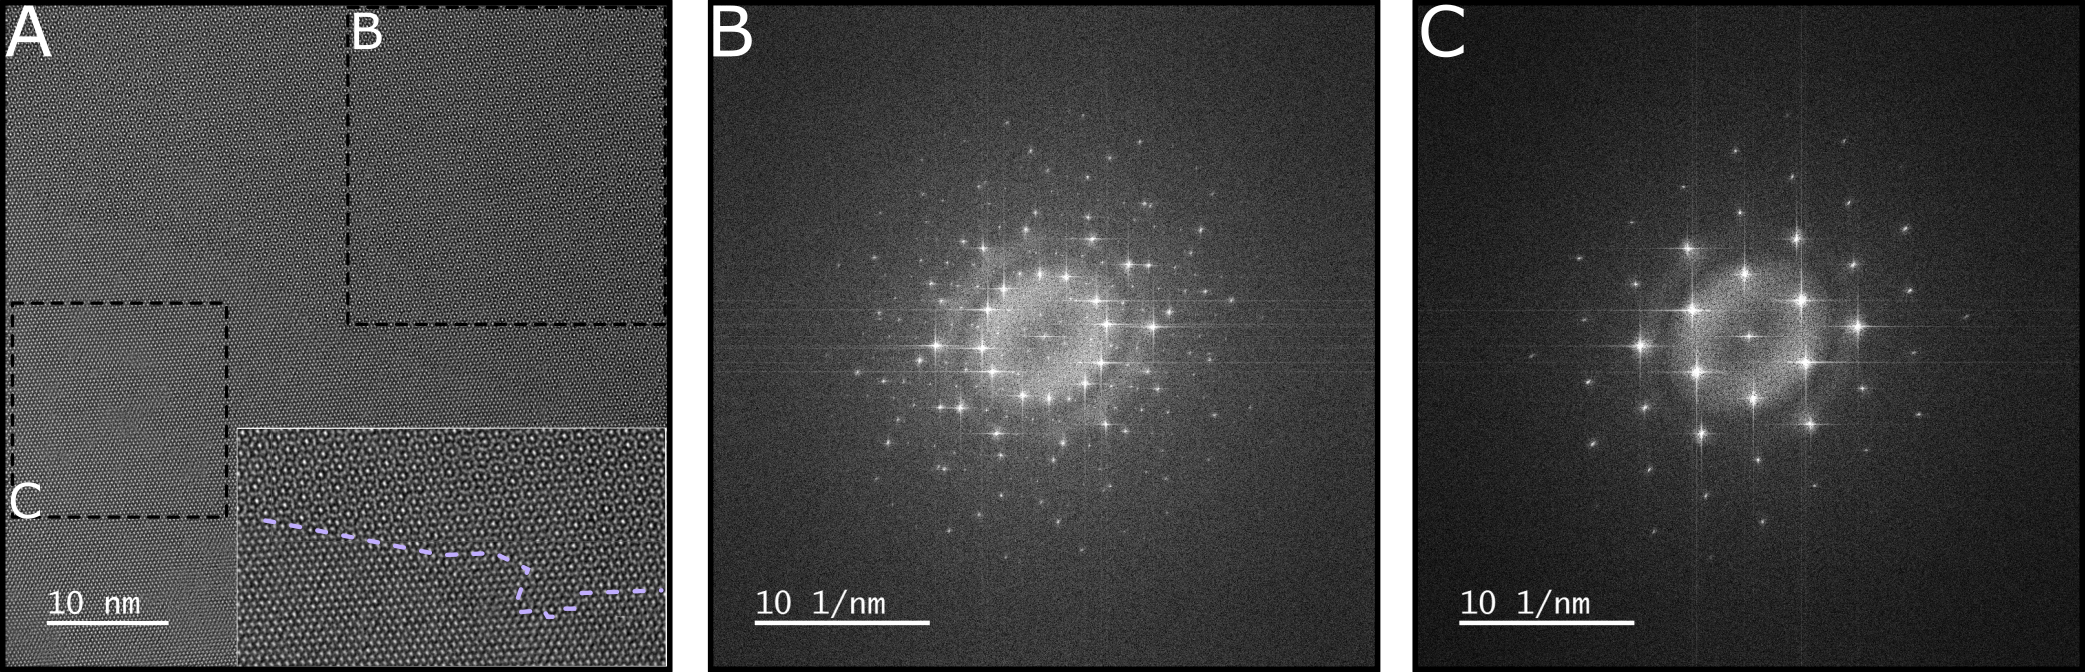
\includegraphics[width=1\linewidth, keepaspectratio]{resources/Figures/moire_transition.png}
    \marginnote{Check detail of Figure \ref{fig:moire_trans}A in print, maybe switch with larger moiré cell} 
    \caption{\textbf{a} High-resolution TEM image of a transition region between singular TMDC material and a twisted heterostructure showing the smallest possible moiré supercell. Dashed regions correspond to subfigures of the same letter, the with white outlined inset is a post-measurement zoomed in image of the transition region with a dashed line guiding the eye towards the flake edge that causes the visual transition. \textbf{b,c} Fast-Fourier transforms of the dashed regions in \textbf{a}. \textbf{b} Shows twelve first-order diffraction peaks indicating that this region consists of two different layers with a roughly \SI{30}{\degree} twist, leading to the smallest possible moiré cell. \textbf{c} Shows six first-order diffraction peaks indicating that its from a single untwisted  crystal. }
    \label{fig:moire_trans}
\end{figure}

Interaction between imaging electrons and crystal lattices lead to the effects described in the previous section, adding a second crystalline structure rotated with respect to the first will affect both lattices as well as create a larger also periodic moiré lattice.
Figure \ref{fig:moire_trans}\textbf{a} shows the transition from single crystal layer to a bilayer region where the constituent layers are rotated from one another, in this bilayer region the effective enlargement of periodic structure is visible as the repeating moiré unit cell is significantly larger than the periodic unit cell of the single layer. The periodicity of the moiré cell is dependent on the rotation between layers and is smallest for \SI{30}{\degree} rotation and increases as the rotation is decreased. The exact periodicity depends on the combination of materials but can be as large as tens of nanometres for transition-metal dichalcogenides with small lattice mismatch \cite{rosenbergerAtomicReconstructionMoire}.

\subsubsection{Diffraction patterns of moiré heterostructures}
The diffraction patterns displayed in Figure \ref{fig:moire_trans}\textbf{b,c} corresponding to the moiré region and the single layer region in Figure \ref{fig:moire_trans}\textbf{a} respectively share some peaks but not all and the extra peaks can not be explained by rotating the diffraction pattern in Figure \ref{fig:moire_trans}\textbf{c} and superimposing in on the pattern in Figure \ref{fig:moire_trans}\textbf{b}.
These extra satellite peaks that emerge between the main Bragg spots and surround the central spot are attributed to the electrons scattering twice, once of off the first layer and then a second time of off the second layer, transferring momentum between the layers while doing so. As these satellite peaks are second order effects they appear dimmer than the main Bragg diffraction spots.
These extra momenta transfer possibilities that open up are displayed schematically in Figure \ref{fig:moire_saed}. In Figure \ref{fig:moire_saed}\textbf{a} the diffraction patterns of two crystal lattice, one red and one blue, are presented; these two lattices each allow six first order momenta transfers by themselves but when brought into proximity the second layer allows scattered electrons to scatter again of its lattice creating the compounded scattering vectors displayed in orange in Figure \ref{fig:moire_saed}\textbf{a,b}. In Figure \ref{fig:moire_saed}\textbf{c} a moiré diffraction pattern is indexed by the cause of the peaks.


\begin{figure}[h]
    \centering
    \def\svgwidth{1\linewidth}
    \import{resources/Figures}{moire_saed.pdf_tex}
    \caption{\textbf{a} Schematic of diffraction patterns of two crystalline samples (red and blue) with a relative twist. The vectors: $\vec{r}_i^n$, $\vec{b}_i^n$, $\vec{c}_i^n$, illustrate the momentum transfers possible due to scattering of a family of planes in the red, blue, or, compound crystal; respectively. In the notation $n$ and $i$ denote the order and the cluster within that order. \textbf{b} Illustration highlighting the new momentum transfer possibilities that open up as two twisted crystalline samples are brought into contact. The newly formed satellite peaks are linear combinations of the intracrystal momentum transfers allowed by the red and/or blue crystal structure and an intercrystal momentum transfers. \textbf{c} Schematic overlaid onto the FFT of a HRTEM image of a moiré cell.}
    \label{fig:moire_saed}
\end{figure}

